\documentclass[a4paper]{report}

\usepackage{amsmath}
\usepackage{amssymb}

\usepackage{alltt}

\usepackage{tikz}

\begin{document}

\title{Thesis Proposal}
\author{Ruud Koot}
\maketitle

% Also see:
% http://www.cs.uu.nl/wiki/bin/view/Thesis/WritingAThesisProposal
% mail from Jur
% Tamar's/Eric's proposal

\chapter*{Introduction}

This document is a proposal for a thesis on answering the research question:
\begin{quote}
Can we use a type and effect system in combination with refinement types to develop a pattern-match analysis for a non-strict higher-order functional language that is both performant and precise enough to be of practical use?
\end{quote}

In Chapter \ref{secmotivation} we present a number of examples to demonstrate why this is an interesting problem. In Chapter \ref{seccontext} we give a short introduction to the relevant concepts of the research question: higher-order functional languages, type and effect systems and refinement types. In Chapter \ref{secrelatedwork} we present work related to our research question and discuss which aspects of that work are relevant to or different from our proposed system. In Chapter \ref{secapproach}, \ref{secdeliverables} and \ref{secevaluation} we will discuss our envisioned approach to answering the research question, the set of deliverables and how we will evaluate whether the research question has been answered successfully or not.

\chapter{Motivation}\label{secmotivation}

In 1978, Robin Milner \cite{Milner78atheory} famously wrote (and proved) that:
\begin{quotation}
Well-typed programs cannot ``go wrong''. 
\end{quotation}
This observation is sometimes
%\footnote{Especially by professors wishing to impress their audience of undergraduate students with the power of types.}
optimistically overstated as ``if your Haskell program type checks and compiles it will work.'' Even if we ignore logic errors, such a strong interpretation of Milner's statement does not hold, as anyone who has seen the dreaded:
\begin{verbatim}
*** Exception: PM.hs:1:1-13: Non-exhaustive patterns in function f
\end{verbatim}
can attest to. To correctly interpret Milner we need to distinguish between three kinds of ``wrongness'':
\begin{description}
\item[Getting stuck] If a program tries to evaluate a non-sensical expression -- such as {\tt 3 + true} -- it cannot possibly make any further progress and is said to be ``stuck''. This is the ``go wrong'' Milner referred to. He proved that a sound type system can statically guarantee such expressions will never occur or need to be evaluated at run-time.
\item[Diverging] If we have a function definition {\tt f = f}, the evaluation of {\tt f} $\leadsto$ {\tt f} $\leadsto ...$ will fail to terminate. We might be making progress in a technical sense, but it will have no useful observable result.
\item[Undefinedness] Another source of ``wrongness'' are partial functions: functions which are not defined on all the elements of their domain. Prime examples are case-statements with missing constructors and functions defined by pattern matching but which do not cover all possible patterns. 
\end{description}

Unlike Milner, who spoke about the first kind of wrongness and the work on termination checking, which concerns itself with the second, we shall focus on the third: a pattern-match analysis which determines if functions are only invoked on values for which they are defined.

% split error and partial definedness?
% loop and crash

\section{Examples}\label{secexamples} % test-driven development

\paragraph{Partial functions} Haskell programmers often work with partial functions, the most common one possibly being {\tt head}:

\begin{verbatim}
1  main = let xs = if length "foo" > 5 then [1,2,3] else []
2          in head xs
3
4  head (x : xs) = x
\end{verbatim}

This program is guaranteed to crash at run-time, so we would like to be warned beforehand by the compiler or a tool:

\begin{verbatim}
On line 2 you applied the function "head" to the empty list "xs".
The function "head" expects a non-empty list as its first argument.
\end{verbatim}

If the guard of the if-statement had read {\tt length "foo" < 5} the program would have run without crashing and we would like the compiler or tool not to warn us spuriously. In case it is not possible to determine statically whether or not a program will crash, a warning should still be raised.

\paragraph{Compiler construction}
Compilers work with large and complex data types to represent the abstract syntax tree. These data structures must be able to represent all syntactic constructs the parser is able to recognize. This results in an abstract syntax tree that is unnecessarily complex and too cumbersome for the later stages of the compiler -- such as the optimizer -- to work with. This problem is resolved by \emph{desugaring} the original abstract syntax tree into a simpler -- but semantically equivalent --  abstract syntax tree than does not use all of the constructors available in the original abstract syntax tree.

The compiler writer now has a choice between two different options: either write a desugaring stage {\tt desugar :: ComplexAST -> SimpleAST} -- duplicating most of the data type representing and functions operating on the abstract syntax tree -- or take the easy route {\tt desugar :: AST -> AST} and assume certain constructors will no longer be present in the abstract syntax tree at stages of the compiler executed after the desugaring step. The former has all the usual downsides of code duplication -- such as having to manually keep the two or more data types synchronized -- while that latter forgoes many of the advantages of strong typing and type safety: if the compiler pipeline is restructured and one of the stages that was originally assumed to run only after the desugaring suddenly runs before that point the error might only be detected at run-time by a pattern match failure. A pattern match analysis should be able to detect such errors statically.

\paragraph{Maintaining invariants}
Many algorithms and data structures maintain invariants that cannot be easily encoded into their type. These invariants often ensure that certain incomplete case-statements are guaranteed not to cause a pattern match failure. An example is the {\tt risers} function from \cite{DBLP:conf/sfp/MitchellR05}, calculating monotonically increasing segments of a list (e.g., {\tt risers [1,3,5,1,2]} $\leadsto$ {\tt [[1,3,5],[1,2]]}):

\begin{verbatim}
1  risers :: Ord a => [a] -> [[a]]
2  risers []         = []
3  risers [x]        = [[x]]
4  risers (x1:x2:xs) = let (s:ss) = risers (x2:xs)
5                       in if x <= y then (x:s):ss else [x]:(s:ss)
\end{verbatim}

The let-binding in the third alternative of {\tt risers} expects the recursive call to return a non-empty list. A naive analysis might raise a warning here. If we think a bit longer, however, we see that we also pass the recursive call to {\tt risers} a non-empty list. This means we will end up in either the second or third alternative in the recursive call. Both the second alternative and both branches of the if-statement in the third alternative result in a non-empty list, satisfying the assumption we made earlier.

Another example might be a collection of mathematical operations working on bitstrings (integers encoded as lists of binary digits without leading zeroes):
\begin{verbatim}
1  type Bitstring = [Int]
2
3  add :: Bitstring -> Bitstring -> Bitstring
4  add [] y = y
5  add x [] = x
6  add (0:x) (0:y) = 0 : add x y
7  add (0:x) (1:y) = 1 : add x y
8  add (1:x) (0:y) = 1 : add x y
9  add (1:x) (1:y) = 0 : add (add [1] x) y
\end{verbatim}

The patterns in {\tt add} are far from complete, but maintain the invariant if passed arguments that satisfy the invariant. So if we are careful to only pass valid bitstrings into a complex mathematical expression of bitstring-operations it will result in a valid bitstring without crashing due to a pattern match failure.

% Examples from Refinement Types for ML:
% * Binary encoded numbers
% * Variable substitutions in Boolean expressions

\chapter{Context}\label{seccontext}

% halting problem
% well-typed programs can't go wrong
% smaller types log form presentation

\section{Haskell}

Haskell is statically-typed functional programming language with non-strict evaluation semantics \cite{Haskell98}. As a functional language it has first-class and higher-order functions and features a rich type system supporting parametric polymorphism and type classes. Programmers can define custom types in the form of algebraic data types and write functions over them using pattern matching.

Like most functional languages, Haskell can be easily translated into a typed $\lambda$-calculus (System $F_C$). From the point-of-view of the programmer it offers a wealth of syntactic sugar over a plain $\lambda$-calculus -- such as guards and list comprehensions -- allowing programs to be expressed concisely and in a readable fashion.

The following example demonstrates the the syntax of Haskell and some features mentioned previously:

\begin{verbatim}
1  data Tree a = Branch (Tree a) (Tree a)
2              | Leaf a
3  
4  mapTree :: (a -> b) -> Tree a -> Tree b
5  mapTree f (Branch t1 t2) = Branch (mapTree f t1) (mapTree f t2)
6  mapTree f (Leaf a)       = Leaf (f a)
7
8  instance Functor Tree where
9      fmap = mapTree
\end{verbatim}
Lines 1--2 define an algebraic data type (ADT) representing a tree. A tree can be constructed by either a {\tt Branch} containing a left and a right subtree or by a {\tt Leaf} containing a value. The ADT is parameterized by a type {\tt a} giving the type of the value stored in the {\tt Leaf}.

Lines 4--5 define a higher-order function {\tt mapTree} which applies a given function {\tt f :: a -> b} to all the values stored in all the leaves of a given {\tt Tree} resulting in a new {\tt Tree}. As the domain and the range of {\tt f} need not coincided the type parameter of the tree changes as well. The body of the function is defined by pattern matching over the constructors of {\tt Tree} and performs recursion in the case of a {\tt Branch} and applies the argument {\tt f} to the field of type {\tt a} in {\tt Leaf} otherwise.

Lines 8--9 declare the type constructor {\tt Tree} to be an instance of the type class {\tt Functor}, expressing it to be an endofunctor in the category of data types with its mapping on morphisms given by {\tt mapTree}.

\subsection{Pattern matching}

Particularly relevant to our analysis are Haskell's pattern matching abilities. We demonstrate some of them in the following function:

\begin{verbatim}
rotate (Branch b@(Branch (Leaf x) (Leaf y)) (Leaf z))
           | z < x     = Branch (Leaf z) b
           | z < y     = Branch (Branch (Leaf x) (Leaf z)) (Leaf y)
           | otherwise = undefined
\end{verbatim}

The function will rotate a tree {\tt (Branch (Branch (Leaf 2) (Leaf 3)) (Leaf 1))} into {\tt Branch (Leaf 1) (Branch (Leaf 2) (Leaf 3))}. It accomplishes this through the use of \emph{nested pattern matching}, \emph{as-patterns} and \emph{guards}.

This function only works on trees of a very specific shape. Feeding the function a tree of a different shape will cause a pattern match failure. Similarly, an error will be raised if the function reaches the {\tt otherwise} branch, containing an {\tt undefined} value. This would also happen if the branch had called {\tt error} or the branch and its guard were left out entirely.

%%%%%%%%%%%%%%%%%%%%%%%%%%%%%%%%%%%%%%%%%%%%%%%%%%%%%%%%%%%%%%%%%%%%%%%%%%%%%%%%

\section{Type and effect systems}

Type and effect systems are approaches to program analysis suitable for typed languages \cite{Nielson:1999:PPA:555142}. In this formalism we take the the \emph{underlying type system} of the language and (conservatively) extend it by adding \emph{annotations} to the types (base, function and other) of the system.

\begin{figure}[p]
\[\frac{}{\Gamma \vdash_{\mathrm{UL}} c : \tau_c}\ \mathrm{[con]} \quad\quad\quad\quad
\frac{\Gamma(x) = \tau}{\Gamma \vdash_{\mathrm{UL}} x : \tau}\ \mathrm{[var]}\]
\[\frac{\Gamma[x \mapsto \tau_1] \vdash_{\mathrm{UL}} e : \tau_2}{\Gamma \vdash_{\mathrm{UL}} \lambda x. e : \tau_1 \to \tau_2}\ \mathrm{[abs]}\]
\[\frac{\Gamma \vdash_{\mathrm{UL}} e_1 : \tau_2 \to \tau_1 \quad \Gamma \vdash_{\mathrm{UL}} e_2 : \tau_2}{\Gamma \vdash_{\mathrm{UL}} e_1\ e_2 : \tau_1}\ \mathrm{[app]}\]
\[\frac{\Gamma \vdash_{\mathrm{UL}} e_1 : \tau_1 \quad \Gamma[x\mapsto \tau_1] \vdash_{\mathrm{UL}} e_2 : \tau_2}{\Gamma \vdash_{\mathrm{UL}} \mathrm{let\ } x = e_1 \mathrm{\ in\ } e_2 : \tau_2}\ \mathrm{[let]}\]
\[\frac{\Gamma \vdash_{\mathrm{UL}} e_1 : \mathrm{bool} \quad \Gamma \vdash_{\mathrm{UL}} e_2 : \tau \quad \Gamma \vdash_{\mathrm{UL}} e_2 : \tau}{\Gamma \vdash \mathrm{if\ } e_0 \mathrm{\ then\ } e_1 \mathrm{\ else \ } e_2 : \tau}\ \mathrm{[if]}\]
\caption{Underlying type system}
\label{underlying}
\end{figure}

\begin{figure}[p]
\[\frac{}{\Gamma \vdash_{\mathrm{AN}} n : \mathrm{int}^{\{n\}}}\ \mathrm{[con]} \quad\quad\quad\quad
\frac{\Gamma(x) = \widehat\tau}{\Gamma \vdash_{\mathrm{AN}} x : \widehat\tau}\ \mathrm{[var]}\]
\[\frac{\Gamma[x \mapsto \widehat\tau_1] \vdash_{\mathrm{AN}} e : \widehat\tau_2}{\Gamma \vdash_{\mathrm{AN}} \lambda x. e : \widehat\tau_1 \to \widehat\tau_2}\ \mathrm{[abs]}\]
\[\frac{\Gamma \vdash_{\mathrm{AN}} e_1 : \widehat\tau_2 \to \widehat\tau_1 \quad \Gamma \vdash_{\mathrm{AN}} e_2 : \widehat\tau_2}{\Gamma \vdash_{\mathrm{AN}} e_1\ e_2 : \widehat\tau_1}\ \mathrm{[app]}\]
\[\frac{\Gamma \vdash_{\mathrm{AN}} e_1 : \widehat\tau_1 \quad \Gamma[x\mapsto \widehat\tau_1] \vdash_{\mathrm{AN}} e_2 : \widehat\tau_2}{\Gamma \vdash_{\mathrm{AN}} \mathrm{let\ } x = e_1 \mathrm{\ in\ } e_2 : \widehat\tau_2}\ \mathrm{[let]}\]
\[\frac{\Gamma \vdash_{\mathrm{AN}} e_1 : \mathrm{bool} \quad \Gamma \vdash_{\mathrm{AN}} e_2 : \tau^{\varphi_2} \quad \Gamma \vdash_{\mathrm{AN}} e_2 : \tau^{\varphi_3}}{\Gamma \vdash_{\mathrm{AN}} \mathrm{if\ } e_0 \mathrm{\ then\ } e_1 \mathrm{\ else \ } e_2 : \tau^{\varphi_2 \cup \varphi_3}}\ \mathrm{[if]}\]
\[\frac{
\Gamma \vdash_{\mathrm{AN}} e : \tau^{\varphi}
}{
\Gamma \vdash_{\mathrm{AN}} e : \tau^{\varphi \cup \varphi'}
}\ \mathrm{[sub]}\]
\caption{Annotated type system}
\label{annotated}
\end{figure}

\subsection{Example}

As an example we give an analysis which determines, in the form of an annotation, which values an expression can evaluate to. The language is the simply-typed $\lambda$-calculus with let-bindings and an if-statement. The underlying type systems is standard and given in Figure \ref{underlying}.

The annotated type system is given in Figure \label{annotated}. It does little more than collecting all constants in the annotations. The only interesting rule is for the if-statement. We need to take the union over the values collected in both branches of the if-statement. We could have chosen to make the rule depend on the annotation of the guard expression, passing on only the values collected in the then-branch along if we knew it could only be {\tt True} or only the values collected in the else-branch if we knew it could only be {\tt False} from its annotation. This would make the analysis more precise.

We have also added an inference rule for \emph{subeffecting}. This allows us to make the annotation less precise. This is sometimes necessary when applying a value about which we have very accurate information to a function which requires a more general argument.

\subsection{Type inference}

An analysis specified as an inference system does not allow us to compute the result of the analysis directly, as the premises of several of the inference rules usually require us to guess the correct type annotations for the type and annotation variables (e.g., in the presence of subeffecting). To overcome this problem we need a \emph{type reconstruction algorithm}.

If the underlying type system is Hindley--Milner, then Algorithm W can be used to infer the types. Algorithm W works bottom-up and can compute types in a single pass by unifying type variables. This may not always be possible for the annotations in an annotated type system, however. Here we can use a variant of Algorithm W to gather a set of constraints on the annotation variables and solve these constraints with a worklist algorithm in a second phase.

\subsection{Polyvariance}

% 1) precision (poisoning)
% 2) modularity

% annotation polymorphism

Consider the following program:
\begin{verbatim}
f = let id x = x
     in (id 1, id 2)
\end{verbatim}

When performing the analysis given above we would assign the type $\mathtt{int} \to \mathtt{int}^{\{1, 2\}}$ to {\tt id} and as a result the type $\mathtt{int}^{\{1,2\}} \times \mathtt{int}^{\{1,2\}}$ to {\tt f}. Clearly, this result is not optimal. This loss in precision has been caused by the two separate calls to {\tt id} \emph{poisoning} each other.

A similar situation occurs at the type-level in the function:
\begin{verbatim}
f = let id x = x
     in (id 1, id true)
\end{verbatim}
Hindley--Milner manages to avoid problems in this situation by a mechanism called \emph{let-generalization}. The binding {\tt id} has the type $\alpha \to \alpha$. Instead of trying -- and failing -- to unify $\alpha$ with both {\tt int} and {\tt bool} in the body of the let-binding, the type of {\tt id} is generalized to the polymorphic type $\forall \alpha. \alpha \to \alpha$. In the body of the let-binding, {\tt id} can be instantiated twice: once to $\mathtt{int} \to \mathtt{int}$ and once to $\mathtt{bool} \to \mathtt{bool}$.

A similar trick can be used for the annotated type system, except that instead of quantifying over type variables, we quantify over annotation variables. 

\section{Refinement types}

\begin{figure}[t]
\centering
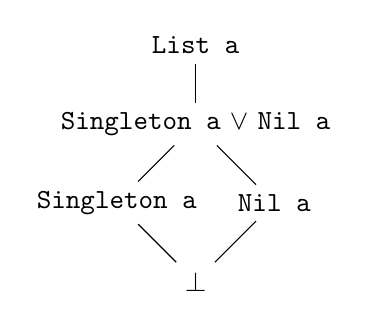
\begin{tikzpicture}
    \tikzstyle{all nodes}=[inner sep=4pt]
    \draw node(top)at(1,3){\tt List a}
          node(sorn)at(1,2){{\tt Singleton a} $\lor$ {\tt Nil a}}
          node(s)at(0,1){\tt Singleton a} node(n)at(2,1){\tt Nil a}
          node(bot)at(1,0){$\bot$};
    \draw[-](top)--(sorn);
    \draw[-](sorn)--(s);
    \draw[-](sorn)--(n);
    \draw[-](s)--(bot);
    \draw[-](n)--(bot);
\end{tikzpicture}
\caption{A lattice of {\tt List} and its {\tt rectype}s.}
\label{listlattice}
\end{figure}


Refinement types are a form of subtyping that allow us to state more accurately what values a variable of a particular type can contain. For example, a refinement type {\tt \{ a :: Int | a < 0 \}} states that {\tt a} is a variable of type {\tt Int} than can only contain negative numbers.

Freeman and Pfenning \cite{Freeman:1991:RTM:113445.113468,Freeman94refinementtypes} give a formal development of refinement types for the ML programming language that can support recursive types.

Their key contribution is allowing the programmer to define {\tt rectype}s. Besides defining a recursive type for lists:

\begin{verbatim}
data List a = Nil | Cons a (List a)
\end{verbatim}

The programmer can also define a {\tt rectype} describing singleton lists:

\begin{verbatim}
rectype Singleton a = Cons a Nil
\end{verbatim}

Together with an automatically derived {\tt rectype} for the non-recurisive constructor {\tt Nil} (and a union type contructor) the compiler can construct -- using known algorithms on regular tree grammars \cite{DBLP:books/others/tree1984} -- a finite lattice of refinement types for {\tt List a} given in Figure \ref{listlattice}.

\subsection{Union and Intersection Types}

Refinement types are constructed from regular types, including function types, as well as union and intersection types.

A union type such as {\tt Int $\lor$ Bool}, {\tt List a $\lor$ Singleton a} or {\tt Int -> Int $\lor$ Bool -> Bool} state a value can be either of the type on the left or of the type on the right, but we do not know which. In the case of {\tt List a $\lor$ Singleton a} we are able to simplify this type to {\tt List a}, as {\tt Singleton a} is a subtype of {\tt List a}.

An intersection type such as {\tt Int $\land$ Bool}, {\tt List a $\land$ Singleton a} or {\tt Int -> Int $\land$ Bool -> Bool} state the a value has both the type on the left and the type on the right. Compared to union types these are more interesting. The type {\tt List a $\land$ Singleton a} can still be simplified, but now to {\tt Singleton a}. A value cannot be of both type {\tt Int} and {\tt Bool}, so we can simply the type of such a value to the bottom or empty type. There do exist functions that are of both type {\tt Int -> Int} and {\tt Bool -> Bool}, for example {\tt id}. In fact, intersection types can in the limit be viewed as a form of parametric polymorphism.

\subsection{Constructors and Pattern Matching}

To infer refinement types more accurate types need to be given to constructors. This is done by using a restricted\footnote{We only take intersections of subtypes of the same data type.} form of intersection types. For example, the {\tt Cons} constructor is given the type:

\begin{verbatim}
Cons :: a -> Nil       a -> Singleton a
     /\ a -> Singleton a -> List      a
     /\ a -> List      a -> List      a
\end{verbatim}

This type can be derived automatically from the {\tt rectype} declarations. Types of functions can also be inferred automatically, although there may be a loss of precision when higher-order functions or polymorphism are involved.

Type inference for intersection types is undecidable in general \cite{Pierce91programmingwith,Reynolds96designof}. Because the lattice of types is finite the algorithm is effectively able to do an exhaustive search over all possible types, however. Higher-order functions can cause the size of the type to blow up exponentially, each pairing of their range and domain needs to be included in the intersection type.

A case-statement 

\begin{verbatim}
case G of
  Nil       -> E1
  Cons a as -> E2
\end{verbatim}

can be seen as a call to a higher-order function

\begin{verbatim}
case_List G E1 (\a as -> E2)
\end{verbatim}

where {\tt case\_list} has the refinement type

\begin{verbatim}
case_List :: forall a. forallR (r1 :: a). forallR (r2 :: a).
       Nil a       -> r1 -> (List a -> r2) -> r1
    /\ Singleton a -> r1 -> (List a -> r2) -> r2
    /\ List a      -> r1 -> (List a -> r2) -> (r1 \/ r2)
\end{verbatim}

\chapter{Related Work}\label{secrelatedwork}

% table comparing the approaches
% * laziness
% * polymorphism
% * annotations (required / supported)
% * decidability
% * errors generated

\section{Neil Mitchell's \emph{Catch}}

Neil Mitchel's \emph{Catch} (``CAse Totality CHecker'') \cite{Mitchell} is a tool specialized in finding potential pattern match failures in Haskell programs.

\subsection{Overview}

Catch works by calculates preconditions on functions. The preconditions are given in a constraint language. By varying the constraint language trade-offs between performance and precision can be made. If the calculated precondition for \texttt{main} is True, the program does not crash.

Preconditions are calculated iteratively. Precondition start out as \texttt{True}, except for \texttt{error}, whose precondition is \texttt{False}.\footnote{Note that {\tt undefined} is defined in terms of {\tt error}.}

\paragraph{Example} Following the example given by Mitchell, given the function:
\begin{verbatim}
safeTail xs = case null xs of
                True  -> []
                False -> tail xs
\end{verbatim}
The computed precondition will be:
\[ \textrm{Precondition}(\texttt{null xs}) \land (\texttt{null xs} \in \{\texttt{True}\} \lor \textrm{Precondition}(\texttt{tail xs})), \]
stating the necessary precondition for \texttt{null xs} not to crash mush be fulfilled and either \texttt{null xs} must evaluate to \texttt{True} or the necessary precondition for \texttt{tail xs} not to crash must be fulfilled.

As \texttt{null xs} cannot crash we find its precondition to be simply True and we can deduce the precondition for \texttt{tail xs} to be $\texttt{xs}\in\{(:)\}$. Substituting these into our precondition we find
\[ \textrm{True} \land (\texttt{null xs} \in \{\texttt{True}\} \lor \texttt{xs}\in\{(:)\}), \]
which simplifies to
\[ \texttt{null xs} \in \{\texttt{True}\} \lor \texttt{xs}\in\{(:)\}. \]
The subexpression  $\texttt{null xs} \in \{\texttt{True}\}$ forms a postcondition on \texttt{null xs}. From this postcondition Catch computes the required precondition that satisfies it, which in this particular case should turn out to be $\texttt{xs}\in\{[]\}$. Substituting, we find
\[ \texttt{xs}\in\{[]\} \lor \texttt{xs}\in\{(:)\}, \]
which, using our knowledge of the list data type, turns out the be a tautology, i.e. the (trivial) precondition for \texttt{safeTail} is True.

\subsection{Constraint systems}
The example in the previous section used a simple constraint language, specifying to which set of head constructors an expression should evaluate. Mitchell developed two more expressive constraint systems: regular expression constraints and multipattern constraints.

\paragraph{Regular expression constraints} Constraints are formed by a regular expression over an alphabet of a number of ad-hoc \emph{selectors} (e.g. \texttt{hd} and \texttt{tl} for lists.) A precondition for \texttt{map head xs} using regular expression constraints reads $\texttt{xs} \in (\texttt{tl}^{*} \cdot \texttt{hd} \leadsto \{(:)\})$. It should be interpreted as ``after applying zero or more \texttt{tl}s to \texttt{xs} and then applying a \texttt{hd} we should find a \texttt{(:)} constructor.''

Accoriding to Mitchell regular expression constraints tend to scale badly as the program increase in size, although he could not identify more specific condition under which this problem manifests.\footnote{Personal communication}

\paragraph{Multipattern constraints} Multipatterns are of the form $\alpha \star \rho$, where $\alpha$ gives the set of constructors that are valid at the head of the value, while $\rho$ gives the set of constructors that can appear at the recursive positions (if any) of the constructor at the head of the value. The elements of these sets can again be multipatterns. To specify that \texttt{xs} in \texttt{map head xs} should be a list of non-empty lists, we use the multipattern:
\begin{align*}
\{[]&, (:) (\{(:)\ \texttt{Any} \} \star \{ [], (:)\ \texttt{Any}\})\} \\
&\star \\
\{[]&, (:) (\{(:)\ \texttt{Any} \} \star \{ [], (:)\ \texttt{Any}\})\}
\end{align*}
\texttt{Any} is a wildcard that matches any constructor.

\subsection{Discussion}
% should have been mentioned earlier?
The analysis of Catch works on a first-order language. The input program needs to be defunctionalized before it can be analyzed. The defunctionalization algorithm employed by Catch is not complete.

Calculated preconditions are unnecessarily restrictive in the presence of laziness (Mitchell, p. 142).


\section{Static Contract Checking}
\subsection{Overview}
Dana Xu's work on static contract checking for Haskell \cite{Xu09staticcontract} (including the ESC/Haskell system \cite{Xu:2006:ESC:1159842.1159849}) allows checking of arbitrary programmer supplied pre- and postconditions on functions and is able to detect pattern match failures in the process.

Programmers define pre- and postconditions in the form of a contract (a refinement type). An appropriate contract for the \texttt{head} function defined above might be:
\begin{verbatim}
{-# CONTRACT head :: {s | not (null s)) -> {x | True} #-}
\end{verbatim}
This contract states that if head is given a list \texttt{s} for which the predicate \texttt{not (null s)} holds, i.e. it is a non-empty list, the function will not crash\footnote{The system only guarantees partial correctness, so the term might still diverge.}, indicated by the trivial postcondition \texttt{True} on the return value.

\begin{figure}
\centering
\begin{tabular}{lclr}
t &$::=$& $\{ x | p \}$     & Predicate          \\
  & $|$ & $x : t_1 \to t_2$ & Dependent function \\
  & $|$ & $(t_1, t_2)$      & Constructor         \\
  & $|$ & $\mathtt{Any}$    & Polymorphic ``Any''
\end{tabular}
\caption{Syntax of Xu's contracts}
\label{xu-contract-syntax}
\end{figure}

Contracts can be constructed from predicates, a dependent function space constructor, arbitrary constructors and a polymorphic \texttt{Any} contract that is always satisfied, including by functions which crash (Fig. \ref{xu-contract-syntax}). Any \texttt{Bool}-valued Haskell expression can be used as a predicate.

Dependent functions are helpful when declaring a contract, e.g. for the \texttt{reverse} function:
\begin{verbatim}
{-# CONTRACT reverse :: {xs | True} -> {rs | length xs == length rs} #-}
\end{verbatim}
The predicate on the return value depends on the the input. Constructors and the \texttt{Any} contract are useful when declaring a contract for \texttt{fst}:
\begin{verbatim}
{-# CONTRACT fst :: (Ok, Any) -> Ok #-}
\end{verbatim}
Here \texttt{Ok} is used as a shorthand for \texttt{\{$x$ | True\}}. As \texttt{fst} discards the value on the right in the tuple we should not care if it is an expression that crashes, so we can not use \texttt{Ok}.

\subsection{Contract checking}
Haskell's syntax is extended with two \emph{exception values} -- \texttt{BAD} and \texttt{UNR} -- which are only used internally by the checker. \texttt{BAD} signifies an expression which crashes and \texttt{UNR} an expression which is either unreachable or diverges.

In the program that is going to be verified all crashing expressions (including \texttt{error} and \texttt{undefined}), as well as missing patterns in case-expressions are replaced by \texttt{BAD} exceptions.

The verification of the contracts is based on a translation of the contracts into Findler--Felleisen wrappers \cite{Findler:2002:CHF:581478.581484}, which will cause a function to crash (using \texttt{BAD}) if it disobeys its contract or diverge if it called in a way that is not permitted. While technically interesting it is not directly relevant to the detection of pattern match failures so we shall not discuss it in more depth.

The actual verification process continues by \emph{symbolic evaluation}, basically applying various simplifications to the resulting program including $\beta$-reductions. Any code deemed to be unreachable is pruned from the program.

The presence of recursive functions in the contracts might cause the symbolic evaluation to diverge if care is not taken to limit the number of evaluation steps. By setting an upper bound on the number of simplification steps we lose accuracy, but gain decidability of the verification process.

Arithmetical expressions in case-expressions (e.g. \texttt{case x*x >= 0 of \{ True -> ...; False -> BAD \}}) cannot be handled directly by the symbolic evaluator. These are collected in a table and send to an external constraint or SMT solver. If the solver determines these expressions are inconsistent the code is unreachable and can be pruned.

After the symbolic evaluation has terminated the checker will tell the programmer if the program is ``definitely satisfies the contract'' (if no \texttt{BAD} exceptions remain anywhere in the program), ``definitely does not satisfy the contract'' or ``don't know.''

\subsection{Discussion}
Unlike our envisioned system, Xu's static contract checking requires programmer supplied contracts on nearly all functions (contracts on trivial functions can be omitted and are handled by inlining their definition when called.) Compared to Mitchell's Catch it can handle higher-order functions natively and has a more (too?) expressive contract language.

\section{Dependent ML}
DML($\mathcal{L}$) is an extension of the ML programming language which enriches ML's type system with a limited form of dependent types over a (decidable) constraint domain (or index language) $\mathcal{L}$ \cite{DML-JFP07}.

Xi's initial example -- recast in a more Haskell-like syntax -- declares a {\tt List} data type dependent on an integer corresponding to the length of the list and a function to concatenate two such lists:
\begin{verbatim}
1  type Nat = {a :: Int | a >= 0}
2
3  data List<Int> a = Nil<0>
4                   | {n :: Nat} Cons<n+1> a (List<n> a)
5
6  (++) :: {m :: Nat} {n :: Nat} List<m> a -> List<n> a -> List<m+n> a
7  (++) Nil         ys = ys
8  (++) (Cons x xs) ys = Cons x (append xs ys)
\end{verbatim}


For many functions producing a list, the exact length might not be derived by such a trivial calculation ({\tt m+n}) on the lengths of the input lists. A prominent example is the {\tt filter} function:
\begin{verbatim}
1  filter :: (a -> Bool) -> {m :: Nat} List<m> a -> [n :: Nat | n <= m] List<n> a
2  filter p Nil         = Nil
3  filter p (Cons x xs) | p x       = Cons x (filter p xs)
4                       | otherwise =         filter p xs
\end{verbatim}
here we only know that the resulting list is equal or shorter in length than the input list ({\tt n <= m}). This is expressed as the dependent sum {\tt [n :: Nat | n <= m]}. In a full-fledged dependently-typed language we would also return a proof object stating the predicate {\tt p} holds for all the elements in the output list, but this is beyond the expressive power of DML.

What we gain is a relief from the need to provide proofs for trivial arithmetical (in)equalities. Imagine a {\tt zip} function which requires the two list to be zipped together to be of equal length. When calling {\tt zip (xs ++ ys) (ys ++ xs)} this preconditions seems to be intuitively satisfied. From the point-of-view of the compiler the first list has length $m+n$ and the second lists $n+m$, however. In most dependently-typed languages we will now have to invoke a lemma or tactic proving the commutativity of addition. DML can simply send the constraint $m + n = n + n$ to an ILP solver and conclude the constraint is satisfiable.

\subsection{Discussion}
Compared to Xu's static contract checking, Xi's DML constrains the constraint system to a decidable theory. The constraints and indices -- such as {\tt m+n} and {\tt n~<=~m} -- may superficially look like ordinary Haskell expression, but in fact belong to a much smaller index language. While type checking is decidable, type inference is not and as a result DML still requires type annotations.

To be applicable to a pattern match analysis we must try to infer a type like:
\begin{verbatim}
head :: {n :: Int | n >= 1} [a]<n> -> a
\end{verbatim}
for the {\tt head} function. We also have to implicitly extend the list data type with an index representing its length.

This seems significantly more challenging than inferring the Catch-like type
\begin{alltt}
head :: \{xs :: [a] | xs \(\in\) (:) \} -> a
\end{alltt}
The correspondence between the the type and the pattern matching happening in the definition of {\tt head} is much more direct.

%\begin{small}
%There is an indirect correspondence, however. The value of the index of the list is given by the {\tt length} function and by analyzing the pattern matching happening in that function we could derive that $\{n :: \mathtt{Int} | n >= 1\}\ \left[a\right]\left<n\right> \simeq \{xs :: [a] | xs \in (:) \}$.
%
%Instead of adding the an index of type {\tt Int} to {\tt List} to create {\tt List<Int>}, we add the abstraction {\tt length :: List -> Int}. This generalizes to arbitrary data types $F$ and constraint systems over $\tau$, by adding an abstraction $F \to \tau$ to create $F\left<\tau\right>$. (But can we use arbitrary functions of type $F\to\tau$, or does {\tt lenght} have some particularly nice properties? Certainly if viewed as a catamorphism (e.g. $(0, (\lambda n. 1+n))$) it should consist of only expressions in the constraint language $\mathcal{L}$ -- they correspond exactly to the annotations on {\tt Nil<0>} and {\tt \{n :: Int\} Cons<n+1>} -- but is this sufficient? What if we look at a {\tt Tree}? Adding a property {\tt minDepth :: Tree -> Int} would guarantee we can pattern match on a certain number of {\tt Branch}es before encountering a {\tt Leaf}, but what does {\tt maxDepth :: Tree -> Int} buy us? More importantly, while we might be able to infer an appropriate type for {\tt head}, inferring the type given to {\tt (++)} and {\tt filter} above still seems out of reach.)
%\end{small}

\section{Compiling Pattern Matching}
Case-statements in toy languages often have a very simple \emph{decision tree} semantics. Case-statements in Haskell have a more complex \emph{backtracking automaton} semantics. There is a body of work on compiling the latter into the former. Maranget \cite{DBLP:journals/jfp/Maranget07} gives an algorithm for determining whether a case-statement is exhaustive and whether all patterns are useful. As the analysis does not consider any dataflow information it is much too imprecise for our purpose. It does turn out that the analysis closely follows, but can at places be simplified with respect to, the manner in which pattern matching is compiled. This indicates might also be able to follow such an approach when analyzing case-statements in our pattern-match analysis.

\chapter{Approach}\label{secapproach}

% type and effect system
% refinement types / subtyping / widening (compare to multi-patterns)
% how much precision do we need?

\section{Incremental development}
We will incrementally develop our analysis for the various constructs in the Haskell language. 

\paragraph{Variables, constants, abstraction, application, if-statements and simple let-bindings} We will start out by implementing the basic constructs of the simply typed $\lambda$-calculus. This includes simple let-bindings, i.e. non-recursive let-bindings in which no pattern matching or generalization occurs. 

At this stage we will only allow booleans and integers as constants. Due to their primitive and infinity nature integers will need to be treated specially by the analysis in any case. Booleans and if-statements can be handles in a more general fashion during later stages.
\paragraph{Recursion} The next elementary construct is recursion. This will require us to implement a form of \emph{widening} for the integers and lists to ensure termination of the analysis. As the exact form of widening used can have a big impact on the precision of the analysis we do not want to commit to a specific lattice here. Various widening strategies should be easily pluggable into the source code and perhaps eventually be able to be specified at a higher-level by the user of the tool.
\paragraph{Simple case-statements} The most critical part of the analysis will be how it handles case-statements. In this state we will add simple case-statements (i.e., non-nested, non-backtracking, guardless case-statements) and primitive list constants, our first recursive data type.
\paragraph{Complex case-statements and guards} To be able to handle the full Haskell 98 language our analysis must be able to deal with the complex semantics of case-statements. This includes nested-patterns, guards and backtracking. We would like to be able to analyze any boolean-valued expression that is used as a guard.
\paragraph{Algebraic data types} Next we extend the analysis to work on arbitrary programmer-defined data types instead of only on our primitive list data type. This will mostly involve generalizing out analysis to work on with a representation of arbitrary algebraic data types. Data types containing fields with function types may also prove interesting.
\paragraph{Polymorphism} Polymorphism can generally be added to an analysis as a relatively orthogonal feature. However, there might be some interesting interactions with our refinement and intersection types here.
\paragraph{Full let-bindings} We extend the analysis for let-bindings to handle (mutual) recursion and pattern matching.
\paragraph{Type classes} An interesting feature of Haskell's type system are type classes. We currently do not foresee any specific difficulties with respect to be able to handle them in out analysis.
\paragraph{Syntactic sugar} As the final stage we would add constructs which are only syntactic sugar and therefore would not pose any significant problem to our analysis. This includes for example list-comprehensions and do-notation.

\section{Refinement types}

Compared to Freeman and Pfenning's approach to refinement types we will initially not rely on programmer supplied, but instead build our lattice of types from finite unrollings of data types. We hope this makes calculating the lattice easier.

Freeman's inference algorithm for refinement type assign a single, albeit complex, type to each binding. This makes it a monovariant analysis. We will develop a polyvariant analysis, making it sensitive to the sites where a binding is used. We hope this will improve the performance of the analysis.

\section{Parsing}

We will develop our tool in the Haskell programming language. A number of libraries for parsing input programs are available. The most obvious choice seem to be the {\tt haskell-src-exts} package, which is also used by the HLint tool. If this proves to be a problematic choice, other possibilities are the parser from GHC or UHC.

\chapter{Deliverables}\label{secdeliverables}

There will be two deliverables of this project:
\begin{enumerate}
\item A \emph{tool} implementing the pattern match analysis for Haskell 98. This tool is intended to be practically usable and not a mere research prototype.
\item A \emph{thesis} describing the theory underlying the tool and documenting the implementation choices made in the tool.
\end{enumerate}

\chapter{Evaluation}\label{secevaluation}

The evaluate whether we were able to answer research question we first need to evaluate whether the developed tool implements a practically usable pattern-match analysis. We can do so by trying it out on the examples sketched in Section \ref{secexamples}, the literature and for example the {\tt nofib} testsuite.

If we can answer this question with a ``yes'', and assuming the tool indeed implements the analysis using a type and effect system and refinement types, we can also answer out research question with a ``yes''.

In case of a ``no'' we will need to argument whether this is due to a failure of our implementation or because there are good theoretical reasons why such an analysis cannot be implemented.

\chapter{Planning}\label{secplanning}

\begin{description}
\item[Implement framework (April)] Implement a constraint-based version of Hindley--Milney for Haskell (the underlying the system of the analysis). This is known work \cite{Odersky:1999:TIC:308181.308203,DBLP:journals/entcs/HageH09} and should not prove to be difficult. This implementation will provide a guiding framework for the analysis, highlight possible issues we might run into when implementing a constraint-based analysis for full Haskell and allow us to decide which parsing library and abstract syntax representation to use.
\item[Implement analysis (April--July)] The largest portion of time is assigned to incrementally developing and building the pattern-match analysis. The likely order will be:
\begin{enumerate}
\item Variables, constants, abstraction, application, if-statements and simple let-bindings (1.5 weeks)
\item Recursion (1.5 weeks)
\item Simple case-statements (2 weeks)
\item Complex case-statements and guards (2 weeks)
\item Algebraic data types (1.5 weeks)
\item Polymorphism (1.5 weeks)
\item Full let-bindings (1 week)
\item Type classes (1.5 weeks)
\item Syntactic sugar (1.5 weeks)
\end{enumerate}
\item[Evaluation and thesis writing (July--August)] The final phase of this project will include an evaluation of the tool and finishing of the thesis. A significant potion of the thesis is expected to be written in parallel with the implementation, after a particular subtask has been implemented successfully.
\end{description}

\chapter{Future Work}

Non-goals of the thesis project are:
\begin{enumerate}
\item A formal soundness proof of the analysis, and
\item Supporting Haskell extensions beyond Haskell 98.
\end{enumerate}
Both of these would be candidates for future work.

\bibliography{thesis-proposal}
\bibliographystyle{plain}

\end{document}
